\cotefile{60}
\scanpage{36}
\begin{center}6 - 31 -\hfill n\textsuperscript{o} 392\end{center}

que $\operatorname{div}_B(Z)$ n'est pas l'image canonique d'un diviseur de $D(A)$. (Raisonner par l'absurde en supposant que $e(\underline{P}/\underline{p})=1$ pour $\underline{P}=BZ$, $\underline{p}=P\cap A$ ; il y aurait alors dans $A$ une uniformisante de $B_{\unsure{P|\underline{P}}}$, nécessairement de la forme $a(X,Y,Z)Z$ avec $b=a(X,Y,0)\ne 0$ ; en déduire que l'on aurait $\Delta b/b=-XY$ et obtenir une contradiction en calculant $\Delta(-XY)$).

24)\quad a) Soient $L$ un corps de caractéristique $2$, $\Delta$ une dérivation de $L$, $K$ le sous-corps de $L$ noyau de $\Delta$ ; on suppose que $[L:K]=2$. Montrer que l'on a $\Delta^2=a\Delta$ avec $a\in K$, et que pour qu'un élément $t\in L$ soit de la forme $\Delta x/x$, il faut et il suffit que $\Delta t=at+t^2$.

b) Soient $B$ un anneau local factoriel de caractéristique $2$, $\underline{m}$ son idéal maximal, $L$ son corps des fractions, $\Delta$ une dérivation de $L$ ; on suppose que le sous-corps $K$ de $L$, noyau de $\Delta$, est tel que $[L:K]=2$ ; en outre, on suppose qu'il existe deux éléments $x$, $y$ de $\underline{m}$ tels que $\Delta x$ et $\Delta y$ engendrent l'idéal $\underline{q}$ de $B$ engendré par $\Delta(B)$. Montrer alors que si $t=\Delta z/z$ appartient à $\underline{q}$, il existe un élément inversible $u$ de $B$ tel que $t=\Delta u/u$, (écrire $t=r\Delta x+s\Delta y$ avec $r$, $s$ dans $B$ et utiliser a)).

25) Soient $k$ un corps de caractéristique $2$, $B$ l'anneau de séries formelles $k[[X,Y]]$, $L$ son corps des fractions, $\Delta$ la $k$-dérivation de $L$ définie par $\Delta(X)=Y^{2j}$, $\Delta(Y)=X^{2i}$, ($i$, $j$ entiers $\geq 0$) ; le sous-anneau $A$ de $B$ formé des $x\in B$ tels que $\Delta x=0$ est l'anneau des séries formelles de $k[[X,Y,Z]]$ où on substitue $X^2$ à $X$, $Y^2$ à $Y$ et $X^{2i+1}+Y^{2j+1}$ à $Z$.

a) Montrer que le groupe $C(A)$ contient un espace vectoriel sur $k$ de dimension $N(i,j)$, égale au nombre des couples d'entiers $(a,b)$ tels que $0\leq a<i$, $0\leq b<j$ et $(2j+1)a+(2i+1)b\geq 2ij$. (Utilisant l'exerc. 23 b) et l'exerc. 24 a), noter que les éléments de $L$ sont les séries formelles $F\in B$ telles que $\Delta F=F^2$ ; en attribuant à $X$ le poids $2j+1$ et à $Y$ le poids $2i+1$, décomposer $F$ en somme infinie de polynômes isobares ; si $L_q$ est le sous-groupe de $L$ formé des $F\in L$ dont les composantes isobares sont de poids $\geq q$, $L/L'$ est isomorphe à la somme directe des groupes $C_q/C_{q+1}$, où $C_q=L_q/(L'\cap L_q)$ ; calculer ces groupes pour $q\geq 4ij$, en utilisant l'exerc. 24 b)).

b) Montrer que l'idéal $AX^2$ de $A$ est premier ; si $A'=A[X^{-2}]$, en déduire que $C(A')$ et $C(A)$ sont isomorphes, (n\textsuperscript{o}\quad, prop.\quad). Montrer que $A'$ est un anneau de Dedekind, (considérer l'anneau $B'=B[X^{-2}]$, qui est entier sur $A'$ et est principal, et utiliser le chap. V, \S\ 2, n\textsuperscript{o} 4, th. 3). En déduire un exemple d'anneau de Dedekind dont le groupe des classes d'idéaux est infini.

\margin{35}

\scanpage{37}
On peut songer à la version additive, en la définissant d'abord sur les $E_{\unsure{\eta|y}}$ simples (i.e. abs. simples, quitte à permettre des extensions finies sur $\mathbf{Q}_{\unsure{\ell|l}}$) et en prolongeant par linéarité, ce qui revient à définir les facteurs locaux d'un $L_{E_{\unsure{\eta|y}}}(\unsure{t})$ par $L_{E_{\unsure{\eta|y}}(x)}(\unsure{t})$, en posant $E_{\unsure{\eta|y}}(x)=\sum E_{\unsure{\eta|y}}^{i*}(x)$, les $E_{\unsure{\eta|y}}^i$ étant les facteurs simples dans une suite de composition de $E$. Ceci n'est pas encore satisfaisant, car les $E_{\unsure{\eta|y}}(x)$ ainsi construits ne sont pas de \unsure{construction} locale en $(E,x)$, -- \unsure{p. ex.} ne commutent pas à l'extension \unsure{étale|ét.} \deleted{sur $X$} (à ext. résiduelle \inserted{en $x$} \deleted{en} triviale) sur $X$.

\margin{36}

\scanpage{38}
\begin{center}6 - 27 -\hfill n\textsuperscript{o} 392\end{center}

12) Démontrer la prop. 5 du n\textsuperscript{o} 8 en utilisant le chap. III, \S\ 2, n\textsuperscript{o} 8, cor. 3 du th. 1.

13) Etendre le cor. de la prop. 7 du n\textsuperscript{o} 8 au cas où l'anneau local séparé et complet $A$ n'est pas intègre, (utiliser \uline{Alg.}, chap. VIII, \S\ 6, exerc. 6 b)).

14) Soient $A$ un anneau local complet noethérien, dont le corps résiduel est de caractéristique $p>0$. Dans l'anneau de séries formelles $A[[T]]$, on considère les éléments $\omega_n=(1-T)^{p^n}$ et $\gamma_n=1-\omega_n$ pour tout entier $n>0$. Montrer que $\gamma_n$ est, au signe près, un polynôme distingué, (n\textsuperscript{o} 8) ; en déduire que $A_n=A[[T]]/(\gamma_n)$ s'identifie à l'algèbre sur $A$ du groupe $G_n=Z/p^nZ$. Montrer que l'intersection des idéaux principaux $(\gamma_n)$ est réduite à $0$ ; en déduire que $A[[T]]$ s'identifie à la limite projective $\varprojlim A_n$.

15) Soient $K$ un corps complet pour une valuation discrète $v$, $A$ l'anneau de la valuation, $k$ son corps résiduel, $P$ un polynôme de $A[X_1,\ldots,X_n]$ de degré total $d$ ayant la propriété suivante : il existe une extension algébrique $K'$ de $K$ telle que dans $K'[X_1,\ldots,X_n]$, $P$ soit produit de polynômes de degré total $1$. On suppose en outre qu'il existe deux polynômes $Q$, $R$ de $A[X_1,\ldots,X_n]$ tels que $Q$ soit de degré total $s$ et contienne un monôme $aX_1^s$ où $\varphi(a)\ne 0$, ($\varphi$ désignant l'homomorphisme canonique $A\longrightarrow k$), que $R$ soit de degré $\leq d-s$, et que l'on ait $\overline{P}=\overline{Q}.\overline{R}$, (notations du chap. III, \S\ 4). Montrer qu'il existe alors dans $A[X_1,\ldots,X_n]$ deux polynômes $Q_0$, $R_0$ de degrés respectifs $s$, $d-s$, tels que $P=Q_0R_0$, $\overline{Q}=\overline{Q}_0$, $\overline{R}=\overline{R}_0$ et que $Q_0$ contienne un monôme $a_0X_1^s$ avec $\varphi(a)=\varphi(a_0)$.

(Considérer $P$, $Q$, $R$ comme des polynômes en $X_1$ à coefficients dans l'anneau $B$, complété de $A[X_2,\ldots,X_n]$ pour la valuation obtenue en prolongeant $v$ suivant la méthode du chap. VI, \S\ 10, n\textsuperscript{o}\quad ; appliquer ensuite le lemme de Hensel ; utiliser enfin l'hypothèse initiale sur $P$).

16) Soient $B$ un anneau de valuation discrète, dont le corps résiduel $k$ est fini et n'est pas un corps premier ; soient $k_0$ le sous-corps premier de $k$, et soit $A$ le sous-anneau de $B$ formé des éléments dont la classe dans le corps résiduel appartient à $k_0$. Soient $\pi$ une uniformisante de $B$, et $(\unsure{\vartheta|\theta}_i)_{1\leq i\leq m}$ un système d'éléments inversibles de $B$ tels que les classes $\overline{\unsure{\vartheta|\theta}}_i$ mod. $\pi$ des $\unsure{\vartheta|\theta}_i$

\margin{37}

\scanpage{39}
\margin{\unsure{NB.} S'il s'agit de \unsure{grps} de type galoisien, et $U$ est ouvert dans $I$, alors il s'ensuit qu'il contient un ss.-grp ouvert \unsure{ds} $U_{\unsure{0}}$, qui est \uline{invariant} dans $D$.}

\uline{\unsure{Sort|Suite} de la \unsure{moyenne}}

$D$ grp., $I$ \unsure{ss.-grp} distingué, $E$ vectoriel de dim finie sur corps $k$, sur lequel $D$ opère. On suppose que $I$ admet un sous-groupe d'indice fini $U$, \inserted{invariant dans $D$,} tel que $g\in U\Rightarrow g$ opère sur $E$ de façon \uline{unipotente}, i.e. valeurs propres \unsure{tous|toutes} $1$. Alors le groupe algébrique d'autom. de $E$ engendré par les $g\in U$ est ``unipotent'', donc \deleted{\illegible{2}} $E$ admet une suite de composition sur $U$ telle que les \inserted{\unsure{$E$ opère} \unsure{triviale|trivialem.} sur les} facteurs \deleted{soient \illegible{1} sur $E$}. De façon précise, on peut prendre la suite de composition par les $E^U$, $(E/E^U)^U$ $\ldots$. Cette suite est stable par les opérations de $D$, \uline{si} \deleted{(comme il est loisible)} \deleted{on prend} \inserted{puisque} $U$ dans $I$ invariant par tout $D$. Donc il existe une suite de composition de $E$ \uline{sur $D$} tels que sur chaque facteur $E_i$, \deleted{$I$} $U$

\margin{38}

\scanpage{40}
\begin{center}6 - 26 -\hfill n\textsuperscript{o} 392\end{center}

à l'intérieur de chaque intervalle, prendre $b_{n+1}=b_nz^{i-1}x^{-1}$ ; à l'extrémité de chaque intervalle, utiliser l'inégalité $ijk-ij-jk-ki\geq 0$).

b) On suppose que $z^{i-1}\notin Ax+Ay$. Montrer qu'il n'existe dans l'anneau $A[[T]]$ aucune série formelle de terme constant $y^k$, ($k$ entier $>0$), et qui soit un élément associé à $v$ dans $B[[T]]$, (calculer le coefficient de $T$ dans le produit de $v$ et d'un élément inversible de $B[[T]]$).

c) Déduire de a), b) et de l'exerc. 7 un exemple d'anneau factoriel $A$ tel que l'anneau de séries formelles $A[[T]]$ ne soit pas factoriel. (Avec les notations précédentes, et en supposant remplies les conditions de a) et b) sur $x$, $y$, $z$, $i$, $j$, $k$, montrer que $vv'$ ne peut être produit de facteurs extrémaux $u_h$, ($1\leq h\leq r$), dans $A[[T]]$ ; on observera que les $u_h$ sont des séries formelles dont les termes constants sont des puissances de $y$. Considérer ensuite l'anneau $C=S'^{-1}A[[T]]$, où $S'$ est formé des séries dont le terme constant est dans $S$ ; $B[[T]]$ est le complété de l'anneau de Zariski $C$ ; montrer que $v'\in C$, et que $v$ et les $u_h$ sont extrémaux dans $C$ ; obtenir finalement une contradiction avec b)).

d) Déduire de c) un exemple d'anneau local factoriel noethérien $A$ dont le complété $\widehat{A}$ est un anneau de Krull non factoriel.

9)\quad a) Soit $A$ un anneau intègre noethérien tel que pour tout idéal maximal $\underline{m}$ de $A$, $A_{\underline{m}}$ soit un anneau de valuation discrète. Si $B$ est l'anneau de séries formelles $A[[X_1,\ldots,X_n]]$, montrer que pour tout idéal maximal $\underline{n}$ de $B$, l'anneau $B_{\underline{n}}$ est factoriel, (considérer son complété, en utilisant la prop. 8 du n\textsuperscript{o} 9). En déduire que tout idéal divisoriel de $B$ est un $B$-module projectif.

b) Soit $C$ un anneau noethérien tel que tout $C$-module projectif de type fini soit libre ; montrer que l'anneau de séries formelles $C[[X]]$ a la même propriété (cf. chap. II, \S\ 3, n\textsuperscript{o} 2, prop. 5).

c) Déduire de a) et b) que si $A$ est un anneau principal, l'anneau de séries formelles $A[[X_1,\ldots,X_n]]$ est factoriel.

10)\quad a) Un anneau factoriel prüférien, (\S\ 2, exerc. 12), est principal.

b) Un anneau de Krull pseudo-bezoutien, (\S\ 1, exerc. 21), est factoriel.

11) Soient $K$ un corps, $A$ l'anneau de polynômes $K[X,Y]$, qui est factoriel ; si $L$ est le corps $K(X^2,Y/X)\subset K(X,Y)$, montrer que l'anneau $A\cap L$ n'est pas factoriel.

\margin{39}

\scanpage{41}
opère trivialt, \inserted{(et réciproquement bien sûr)} Donc \unsure{du pt de} vue virtuel, \inserted{et pour $U$ fixé,} les modules $E$ envisagés sont \unsure{essentiellement} les \unsure{$=$s|mêmes} que les modules tels qu'\deleted{il existe un ss-grp \unsure{tel que}} $U$ opère trivialt sur $E$.

Or pour un $E$ sur lequel $U$ opère trivialt, on peut prendre l'opération moyenne
\[
E\leadsto E^I\qquad\text{de}\quad \operatorname{Mod}(D/U,k)-\operatorname{Mod}(D/I,k)
\]
et si $k$ est de car. $0$, c'est là un \deleted{opération \uline{additive}, qui \unsure{nous donne}} \inserted{foncteur exact. Il induit un hom.} \deleted{\unsure{de gr.}} virtuel \deleted{$\unsure{E}$} $E\leadsto E^{\unsure{\natural|\xi}}$
\[
\unsure{\natural|\xi}_U:\ R(D/U,k)\longrightarrow R(D/I,k)
\]
On a. compatibilité, pour $V\subset U$, pour les \uline{foncteurs} $E\leadsto E^I$, d'où pour les $\unsure{\natural|\xi}_U$ et $\unsure{\natural|\xi}_V$ :
\diagram{\begin{tikzcd}[column sep=large,row sep=large]
R(D/U,k) \arrow[r,no head,"{\unsure{\natural|\xi}_U}"] \arrow[d,"{\text{\uline{\unsure{restr.}}}\ \deleted{\unsure{\natural}}}"'] & R(D/I,k) \\
R(D/V,k) \arrow[ur,"{\unsure{\natural|\xi}_V}"'] &
\end{tikzcd}}

\margin{40}

\scanpage{42}
\begin{center}6 - 25 -\hfill n\textsuperscript{o} 392\end{center}

c)\unsure{.}Soient $k$ un corps ordonné, $a$, $b$ des éléments $>0$ de $k$ et $B$ l'anneau $k[X,Y]/(aX^2+bY^2+1)$. Montrer que $B$ est un anneau factoriel, (utiliser b) et l'exerc. 17 a) du \S\ 1).

d) Montrer que l'anneau $C=Q[X,Y]/(X^2+2Y^2+1)$ est factoriel, mais que l'anneau $C\otimes_Q Q(i)$, (avec $i^2=-1$), n'est pas factoriel.

7) Soient $K$ un anneau factoriel noethérien, $F$ un élément extrémal de l'anneau de polynômes $K[X_1,\ldots,X_n]$ ; on suppose que lorsque l'on attribue à chaque $X_i$ un poids $q(i)>0$, ($1\leq i\leq n$), $F$ est isobare et de poids $q>0$. Soit $A$ l'anneau engendré, dans une clôture algébrique $\Omega$ de $K(X_1,\ldots,X_n)$ par $K$, les $X_i$, ($1\leq i\leq n$), et une racine $z$ du polynôme $Z^c-F$, où $c$ est un entier étranger à $q$. Montrer que $A$ est factoriel dans les deux cas suivants :

1) on a $c\equiv 1$ (mod. $q$) ;

2) tout $K$-module projectif de type fini est libre, (ce qui a lieu par exemple lorsque $K$ est un corps, ou un anneau principal, ou un anneau local).

(Dans le premier cas, considérer l'anneau de fractions $A[1/z]$ ; montrer qu'il est factoriel et appliquer la prop. 3 du n\textsuperscript{o} 4. Dans le second cas, considérer un entier $d$ tel que $cd\equiv 1$ (mod. $q$), et soit $z'\in\Omega$ tel que $z=z'^{d}$ ; l'anneau $B=A[z']$ est factoriel en vertu du premier cas, et est un $A$-module libre. Considérer $B$ comme un anneau gradué en prenant $z'$ de poids $q$, chacun des $X_i$ de poids $cdq(i)$, et se ramener à prouver que pour deux éléments homogènes $u$, $v$ de $A$, l'idéal $Au\cap Av$ est principal, en utilisant l'exerc. 16 du \S\ 1 ; considérer enfin l'idéal $Bu\cap Bv$ dans $B$ et utiliser le chap. I, \S\ 3, n\textsuperscript{o} 6, prop. 12). En particulier, si $K$ est un corps, $a$, $b$, $c$ trois entiers $>0$ étrangers deux à deux, l'anneau $A=K[X,Y,Z]/(Z^a-X^b-Y^c)$ est factoriel.

8) Soient $A$ un anneau intègre, $x$, $y$, $z$ trois éléments non nuls de $A$ où $x$ est extrémal et $Ax\cap Ay=Axy$. Soit $S$ l'ensemble multiplicatif des $x^n$, ($n\geq 0$), et soit $B=S^{-1}A$ ; on considère les anneaux de séries formelles $A[[T]]$ et $B[[T]]$.

a) Soient $i$, $j$, $k$ trois entiers $\geq 0$ tels que $ijk-ij-jk-ki\geq 0$ et $z^i\in Ax^j+Ay^k$. On considère dans $A[[T]]$ l'élément $v=xy-z^{i-1}T$. Montrer qu'il existe un entier $t>0$ et une série $v'=y^tx^{-1}+b_1x^{-2}T+\ldots\ \ldots+b_{n-1}x^{-n}T^{n-1}+\ldots$ dans $B[[T]]$ tels que $vv'\in A[[T]]$, (on déterminera par récurrence les $b_n$, en procédant dans $N$ par intervalles de longueur $ij$ ;

\margin{41}

\scanpage{43}
D'autre part, on a
\[
R(D/U\ k)\hookrightarrow R(D,k)
\]
et l'image de $R(D/U,k)$ dans $R(D,k)$ est précisément formée des classes \unsure{des|de} $E$ satisfaisant la condition du début. Pour un tel $E$, on a donc une opération $\unsure{\natural|\xi}$ sur la \uline{classe} de $E$. Donc $\operatorname{cl}(E)^{\unsure{\natural|\xi}}$ est défini dès qu'il existe un ss-grp \deleted{\unsure{distingué|d'indice}} $U$ d'indice fini dans $I$ tel que \deleted{$D/U$} $U$ opère sur $E$ de façon unipotente. / Si on prend des classes de repr. \uline{continues} ($k$ étant un corps top) on \deleted{prend} \inserted{obtient} des \deleted{$\unsure{=}$} $\operatorname{cl}(E)^{\unsure{\natural|\xi}}$ comme classes de repr. \uline{continues} de $D/I$. Compatibilité avec ext des corps de base.

\deleted{Supposons que $D/I\simeq\mathbf{Z}$, et \unsure{donc} qu'une classe de repr. sur $D/I$ est donnée par sa série car. - $L_{E^{\unsure{\natural|\xi}}}(t)$. On aura alors}

\margin{42}

\scanpage{44}
\begin{center}6 - 24 -\hfill n\textsuperscript{o} 392\end{center}

4)\quad a) Montrer que l'anneau $A=Q[X,Y]/\underline{p}$, où $\underline{p}$ est l'idéal principal engendré par $X^2+Y^2-1$ dans $Q[X,Y]$, est un anneau de Krull non factoriel, (montrer que $X$ est un élément extrémal de $A$ mais que $AX$ n'est pas un idéal maximal de $A$).

b) Montrer que l'anneau $A\otimes_Q Q(i)$ est factoriel, (prouver que cet anneau est isomorphe au quotient de $Q(i)[X,Y]$ par l'idéal principal $(XY-1)$ ; comparer à l'exerc. 3 b)).

5)\quad a) Soient $k$ un anneau factoriel noethérien, $B$ l'anneau de polynômes $k[X_1,\ldots,X_n]$ avec $n\geq 3$ ; soient $g_i$, ($0\leq i\leq r$), des éléments de $k[X_3,\ldots,X_n]$ où $g_0$ est extrémal. On pose $g=X_1X_2-\sum_{i=0}^r g_iX_1^i$, et on considère l'anneau quotient $A=B/gB$. Montrer que $A$ est factoriel. (Soit $S$ la partie multiplicative de $A$ engendrée par $1$ et l'image de $X_1$ dans $A$ ; appliquer à $S^{-1}A$ la prop. 3 du n\textsuperscript{o} 4).

b) Soient $k$ un corps de caractéristique $\ne 2$, $F$ un polynôme homogène du second degré de $k[X_1,\ldots,X_n]$ avec $n\geq 5$, tel que la fonction polynôme correspondante sur $k^n$ soit une forme quadratique non dégénérée. Montrer que l'anneau $k[X_1,\ldots,X_n]/(F)$ est factoriel. (On prouvera d'abord qu'un polynôme homogène $G$ du second degré dans $k[X_1,\ldots,X_n]$ tel que la fonction polynôme correspondante soit une forme quadratique non dégénérée, est extrémal pour $n\geq 3$. Prouver ensuite la proposition lorsque $k$ est algébriquement clos, en utilisant a) ; passer enfin au cas général à l'aide de l'exerc. 3 b)).

c) Si $F=X_1X_2-X_3X_4$, montrer que l'anneau $k[X_1,X_2,X_3,X_4]/(F)$ n'est pas factoriel. (Montrer que les images des $X_i$ dans cet anneau sont des éléments extrémaux).

6)\quad a) Soit $K$ un corps algébriquement clos de caractéristique $\ne 2$. Déterminer les idéaux premiers gradués de l'anneau $K[X,Y,Z]/(X^2+Y^2+Z^2)$.

b) Soient $k$ un corps ordonné, $a$, $b$, $c$ des éléments $>0$ de $k$ et $A$ l'anneau $k[X,Y,Z]/(aX^2+bY^2+cZ^2)$. Montrer que $A$ est un anneau factoriel. (Se ramener au cas où $k$ est un corps ordonné maximal, en utilisant l'exerc. 3 b) ; prouver alors, en utilisant a), que tout idéal premier gradué de hauteur $1$ dans $A$ est principal, et appliquer l'exerc. 3 a)).

\margin{43}

\scanpage{45}
Calculons la \uline{trace} de la représentation \unsure{dérivée}, on trouve pour $\varphi\deleted{\unsure{\xi}}\in D/I$
\[
\operatorname{Tr}_{E^{\unsure{\natural|\xi}}}(\varphi)\deleted{\unsure{\xi}}=\sum_i\operatorname{Tr}_{E_i^{\unsure{\natural|\xi}}}(\varphi)
\]
Or si \deleted{$I$} $U$ opère trivialt sur $E$, \deleted{qui est} alors un module sur $D/U$, on a
\[
E^{\unsure{\natural|\xi}}=\operatorname{Im}\deleted{\unsure{\xi}}\pi_{\deleted{\unsure{I}}}\inserted{\text{projection}}\qquad
\pi=\frac{1}{N}\sum_{i\in I/U}e_i.\quad N=\operatorname{card} I/U
\]
donc si $g\in\unsure{I|D}/U\longrightarrow\varphi$ on a
\[
\operatorname{Tr}_{E^{\unsure{\natural|\xi}}}(\varphi)=\operatorname{Tr}_E(\deleted{\unsure{I}}\pi g)\deleted{=\frac{1}{N}\sum_{\substack{g\to\varphi\\\unsure{g\in I}}}\operatorname{Tr}_E(}
\]
d'où
\[
\boxed{\operatorname{Tr}_{E^{\unsure{\natural|\xi}}}(\varphi)=\frac{1}{N}\sum_{\substack{\psi_\alpha\in D/U\\\deleted{\unsure{g}}\\\psi_\alpha\to\varphi\in D/I}}\operatorname{Tr}_E\psi_\alpha}
\]
Comme \inserted{les deux mb. de} cette formule sont linéaires en $E$, ceci reste valable pour \unsure{tt} $E$ ; il faut simplement noter que $\operatorname{Tr}_E\psi$ est défini \deleted{\unsure{sur}} pour $\psi\in D/U$, si $U$ opère de façon unipotente, comme $\operatorname{Tr}_E(\psi')$ pour $\psi'\in D$ \unsure{se relevant} en $\psi$ : cette valeur ne \uline{dépend pas} du

\margin{44}

\scanpage{46}
\begin{center}4 - 42 -\hfill n\textsuperscript{o} 392\end{center}

morphe à un idéal de $A$. Supposons donc $n\geq 2$ ; en vertu du lemme 8, il existe un sous-module libre $L_0$ de $M$, de rang $1$, tel que $M/L_0$ soit sans torsion ; $M/L_0$ est donc de rang $n-1$. En vertu de l'hypothèse de récurrence, il y a donc un sous-module libre $L_1$ de $M/L_0$ tel que $(M/L_0)/L_1$ soit isomorphe à un idéal de $A$. Soit $L$ l'image réciproque de $L_1$ dans $M$ ; $L/L_0$ est isomorphe à $L_1$, et puisque $L_1$ est libre, $L$ est isomorphe à $L_0\oplus L_1$, (\uline{Alg.}, chap. II, 3e éd., \S\ 1, n\textsuperscript{o} 11, prop. 21), donc libre ; comme $M/L$ est isomorphe à $(M/L_0)/L_1$, le théorème est démontré.

\uline{Remarque}.- Si $M$ est réflexif, il n'en est pas nécessairement de même de $M/L$, (exerc.\quad).

10. \uline{Modules sur les anneaux de Dedekind}.

On suppose maintenant que $A$ soit un \uline{anneau de Dedekind} ; on sait alors que les idéaux $\underline{p}\in P$ sont \uline{maximaux} et que ce sont les seuls idéaux premiers $\ne 0$ de $A$, (\S\ 2, n\textsuperscript{o} 2, th. 1) ; le groupe $D(A)$ s'identifie au groupe $I(A)$ des idéaux fractionnaires $\ne 0$ de $A$.

PROPOSITION 21.- \uline{Soit} $A$ \uline{un anneau de Dedekind}. \uline{Tout} $A$-\uline{module pseudo-nul est nul}. \uline{Tout homomorphisme pseudo-injectif}, (resp. \uline{pseudo-surjectif}, \uline{pseudo-bijectif}, \uline{pseudo-nul}), \uline{de} $A$-\uline{modules est injectif}, (resp. \uline{surjectif}, \uline{bijectif}, \uline{nul}).

La première assertion a déjà été démontrée, (n\textsuperscript{o} 4, \uline{Exemple} 1) ; les autres s'en déduisent immédiatement.

PROPOSITION 22.- \uline{Soient} $A$ \uline{un anneau de Dedekind}, $M$ \uline{un} $A$-\uline{module de type fini}. \uline{Les propriétés suivantes sont équivalentes} :

a) $M$ \uline{est sans torsion}.

b) $M$ \uline{est réflexif}.

c) $M$ \uline{est projectif}.

On sait déjà, (sans hypothèse sur l'anneau intègre $A$), que b) implique a), (n\textsuperscript{o} 2, \uline{Remarque} 1), et que c) implique b), (\uline{Alg.}, chap. II, 3e éd., \S\ 2, n\textsuperscript{o} 7,

\margin{45}

\scanpage{47}
choix de $\psi'$ relevant $\psi$, comme on voit à l'aide de la suite de composition.

\figure{\begin{tikzpicture}\draw (0,0)--(3,0);\end{tikzpicture}}

Revenons au cas géométrique, en prenant pour $D$ le grp de décomposition $D_x$ d'un $x\in X$, $I$ le grp d'inertie, donc $D_x/I_x\simeq\unsure{\Pi|\pi}_x\simeq\widehat{\mathbf{Z}}$ (générateur $\unsure{f_x|F_x}$). On posera
\[
E_{\unsure{\eta|y}}(x)=E_{\unsure{\eta|y}}^{\unsure{\natural|\xi}(x)}\qquad\text{comme module sur }\unsure{\Pi|\pi}_x.
\]
\deleted{On pourra}

\unsure{Il revient|Il vient} au \unsure{$=$|même}, du pt de vue faisceau virtuel sur $X$, de poser
\[
E_{\unsure{\eta|y}}^{\unsure{\natural|\xi}}=i_!(E_U)+\sum_{x\in Y}j_{x*}\bigl(E_{\unsure{\eta|y}}^{\unsure{\natural|\xi}(x)}\bigr)
\]
où $U$ est un ouvert dense de $X$ sur lequel $E_{\unsure{\eta|y}}$ n'est pas ramifié, $E_U$ est le \unsure{prolg} de $E_{\unsure{\eta|y}}$ sur $U$, \inserted{$Y=X-U$,} $i:U\mathrel{\text{---}}X$ \inserted{et $j:Y\mathrel{\text{---}}X$} les immersions canoniques,
\[
j_x:\operatorname{Spec} k(x)\longrightarrow X.
\]

\margin{46}

\scanpage{48}
\begin{center}4 - 41 -\hfill n\textsuperscript{o} 392\end{center}

principal semi-local, dont les idéaux maximaux sont les $\underline{p}S^{-1}A$, où $\underline{p}\in Y$, les anneaux locaux correspondants étant les $A_{\underline{p}}$. On a donc $S^{-1}A/\underline{p}S^{-1}A=k(\underline{p})$, d'où $S^{-1}M/\underline{p}S^{-1}M=(M/\underline{p}M)\otimes_A S^{-1}A=M\otimes_A(A/\underline{p}\otimes_A S^{-1}A)=M\otimes_A k(\underline{p})=M(\underline{p})$ pour tout $\underline{p}\in Y$. En vertu du chap. II, § 1, n\textsuperscript{o} 2, prop. 6, il existe un élément $z/s\in S^{-1}M$, $(z\in M,s\in S)$, dont les images canoniques dans les $M(\underline{p})$ pour $\underline{p}\in Y$ sont toutes $\ne0$. Par définition de $S$, on a donc $z(\underline{p})\ne0$ pour tout $\underline{p}\in Y$. On peut en outre supposer que $y$ et $z$ sont \uline{linéairement indépendants} sur $K$. En effet, dans le cas contraire, considérons un élément $t\in M$ linéairement indépendant de $y$, (il en existe puisque $n\ge2$) ; prenons d'autre part un élément $a\ne0$ appartenant à $\bigcap_{\underline{p}\in Y}\underline{p}$, (qui n'est pas réduit à $0$ puisque $A$ est intègre), et posons $z'=z+at$ : il est clair que $y$ et $z'$ sont linéairement indépendants sur $K$ et que l'on a $z'(\underline{p})=z(\underline{p})\ne0$ pour tout $\underline{p}\in Y$.

Supposant donc $y$ et $z$ linéairement indépendants sur $K$, soit $Z$ l'ensemble des $\underline{p}\in P-Y$ tels que $y(\underline{p})$ et $z(\underline{p})$ soient linéairement dépendants sur $k(\underline{p})$ ; il résulte du lemme 7 que cet ensemble est \uline{fini}. Pour tout $\underline{p}\in Z$, on peut donc écrire $z(\underline{p})=\lambda(\underline{p})y(\underline{p})$ avec $\lambda(\underline{p})\in k(\underline{p})$. Or, on a $\operatorname{Card}(A/\underline{p})\ge2$ pour tout $\underline{p}\in P$ ; il résulte donc du lemme 6 qu'il existe $b\in A$ tel que, pour tout $\underline{p}\in Z$, l'image canonique de $b$ dans $A/\underline{p}$ soit distincte de $\lambda(\underline{p})$. Montrons alors que l'élément $x=z-by$ répond à la question ; il suffit, (en vertu du lemme 7 appliqué pour $m=1$), de vérifier que $x(\underline{p})\ne0$ pour \uline{tout} $\underline{p}\in P$. Or :

- si $\underline{p}\in Y$, on a $x(\underline{p})=z(\underline{p})\ne0$ par construction ;

- si $\underline{p}\in Z$, on a $x(\underline{p})=\mu_{\underline{p}}.y(\underline{p})$ avec $\mu_{\underline{p}}\ne0$ en vertu du choix de $b$, donc $x(\underline{p})\ne0$ puisque $y(\underline{p})\ne0$ ;

- si $\underline{p}\in P-(Y\cup Z)$, $y(\underline{p})$ et $z(\underline{p})$ sont linéairement indépendants, donc $x(\underline{p})\ne0$.

Ces lemmes étant établis, passons à la démonstration du th. 6. Raisonnons par récurrence sur $n$, le cas $n\le1$ étant trivial puisque $M$ lui-même est alors iso-

\margin{47}
\scanpage{49}
Calcul de $D(E_{\unsure{\eta|y}}^{\unsure{\natural|\xi}})$ :

\[
\begin{aligned}
D(E_{\unsure{\eta|y}}^{\unsure{\natural|\xi}})
&=D(i_!(E_U))+\sum_{x\in Y}D(j_{x*}(E_{\unsure{\eta|y}}^{\unsure{\natural|\xi}(x)}))\\
&=\unsure{\mathbb{R}|\mathbf{R}}i_*(DE_U)+\sum_{x\in Y}j_{x*}(D(E_{\unsure{\eta|y}}^{\unsure{\natural|\xi}(x)}))
\end{aligned}
\]

Or la formation de $\unsure{\natural|\xi}$ \unsure{local} commute au \unsure{passage au} dual, d'autre part on a
\[
D(E_U)=\check E_U(1)\deleted{[2]\unsure{E_U(\varphi+1)|E_U(\rho+1)}},
\]
d'où
\[
\begin{aligned}
D(E_{\unsure{\eta|y}}^{\unsure{\natural|\xi}})
&=(\unsure{\mathbb{R}|\mathbf{R}}i_*(\check E_U))(\deleted{\unsure{\varphi|\rho}}1)+\sum_{x\in Y}j_{x*}(\check E_{\unsure{\eta|y}}^{\unsure{\natural|\xi}(x)})\\
&\deleted{\unsure{=}}\\
&=\unsure{\mathbb{R}|\mathbf{R}}i_!(\deleted{\unsure{i_*}}\check E_U)(\deleted{\unsure{\varphi|\rho}}1)+\sum_{x\in Y}\deleted{\unsure{\{}}j_{x*}\bigl[\check E_{\unsure{\eta|y}}^{\unsure{\natural|\xi}(x)}\deleted{\unsure{)}}+j_x^*\unsure{\mathbb{R}|\mathbf{R}}i_*(\check E_U)(1)\bigr]\\
&=\check E_{\unsure{\eta|y}}^{\unsure{\natural|\xi}}(1)+\sum_{x\in Y}j_{\unsure{x*|*x}}(\mu_{\deleted{\unsure{\eta}}x}(E))
\end{aligned}
\]
\deleted{Il y a donc}

\[
\mu_x(E)=\check E_{\unsure{\eta|y}}^{\unsure{\natural|\xi}(x)}\unsure{\otimes}(\deleted{\unsure{1}}\mathbf{Q}_\ell-\mathbf{Q}_\ell(1))+j_x^*\unsure{\mathbb{R}|\mathbf{R}}i_{\unsure{\eta|y}*}(\check E_{\unsure{\eta|y}})(1)
\]
\deleted{$\unsure{=\check E_{\unsure{\eta|y}}^{\unsure{\natural|\xi}(x)}}$}

Or \unsure{par} dualité locale, on a \deleted{\unsure{par local}}
\[
j_x^*(\unsure{\mathbb{R}|\mathbf{R}}i_{\unsure{\eta|y}}(\check E_{\unsure{\eta|y}}))=\check E_{\unsure{\eta|y}\deleted{\unsure{x}}}(x)-(E_{\unsure{\eta|y}}(x))^\vee(-1)
\]

\margin{48}
\scanpage{50}
\begin{center}4 - 40 -\hfill n\textsuperscript{o} 392\end{center}

\uline{indépendants sur} $k(\underline{p})$ ; \uline{pour qu'ils soient linéairement indépendants sur} $k(\underline{p})$ \uline{pour tout} $\underline{p}\in P$, \uline{il faut et il suffit que} $M/L$ \uline{soit sans torsion}.

Soient $x_{m+1},\ldots,x_n$ des éléments de $M$ qui, avec $x_1,\ldots,x_m$, forment une base de $V$, et soit $N$ le sous-$A$-module libre de $M$ engendré par les $x_i$, $(1\le i\le n)$. Il résulte du n\textsuperscript{o} 3, th. 3 que l'on a $N_{\underline{p}}=M_{\underline{p}}$ pour presque tout $\underline{p}\in P$ ; comme $x_1(\underline{p}),\ldots,x_n(\underline{p})$ forment une base de $N(\underline{p})$ sur $k(\underline{p})$, cela établit la première assertion.

Si $M/L$ est sans torsion, il en est de même \unsure{dc|de} $(M/L)_{\underline{p}}=M_{\underline{p}}/L_{\underline{p}}$ pour tout $\underline{p}\in P$, (n\textsuperscript{o} 1, \uline{Exemple} 6), et comme $A_{\underline{p}}$ est principal, $M_{\underline{p}}/L_{\underline{p}}$ est libre. Par suite, $M_{\underline{p}}$ est somme directe de $L_{\underline{p}}$ et d'un $A_{\underline{p}}$-module libre $E$ de rang $n-m$ ; donc $M(\underline{p})$ est somme directe de $L(\underline{p})$ et du $k(\underline{p})$-espace vectoriel $E/\underline{p}E$, de dimension $n-m$ ; par suite $L(\underline{p})$ est de dimension $m$, et comme il est engendré par les $x_i(\underline{p})$, $(1\le i\le m)$, ces derniers sont linéairement indépendants.

Inversement, supposons que les $x_i(\underline{p})$, $(1\le i\le m)$, soient linéairement indépendants sur $k(\underline{p})$ pour tout $\underline{p}\in P$. Alors $L_{\underline{p}}$ est facteur direct de $M_{\underline{p}}$ pour tout $\underline{p}$, (chap. II, § 3, n\textsuperscript{o} 2, cor. 1 et 2 de la prop. 5), et par suite $M_{\underline{p}}/L_{\underline{p}}=(M/L)_{\underline{p}}$ est sans torsion pour tout $\underline{p}\in P$. On en conclut que $P\cap\operatorname{Ass}(M/L)=\varnothing$ en vertu du chap. IV, § 1, n\textsuperscript{o} 2, cor. de la prop. 5. Mais comme $L$ est réflexif, il résulte du n\textsuperscript{o} 2, prop. 6, (i), que le seul idéal premier qui puisse appartenir à $\operatorname{Ass}(M/L)$ est l'idéal $(0)$ ; donc $M/L$ est sans torsion.

LEMME 8.- \uline{Supposons que le rang} $n$\unsure{-}\uline{de} $M$ \uline{soit} $\ge2$ ; \uline{alors il existe un élément} $x\ne0$ \uline{de} $M$ \uline{tel que} $M/Ax$ \uline{soit sans torsion}.

Soit $y\ne0$ un élément de $M$. En vertu du lemme 7, l'ensemble $Y$ des $\underline{p}\in P$ tels que $y(\underline{p})=0$ est fini. Si $Y=\varnothing$, il résulte du lemme 7 appliqué à la suite $(x_i)$ formée du seul élément $y$, que $M/Ay$ est sans torsion. Supposons donc $Y\ne\varnothing$, et posons $S=\bigcap_{\underline{p}\in Y}(A-\underline{p})$ ; on sait, (n\textsuperscript{o} 4, lemme 2), que $S^{-1}A$ est un anneau

\margin{49}
\scanpage{51}
Posons
\[
\boxed{\alpha_x(E_{\unsure{\eta|y}})=E_{\unsure{\eta|y}}^{\unsure{\natural|\xi}(x)}-E_{\unsure{\eta|y}}(x)}
\]
Alors
\[
\boxed{\mu_x(E)=\alpha_x(E_{\unsure{\eta|y}})^\vee-\alpha_x(\check E_{\unsure{\eta|y}})(1)}
\]

[\unsure{car}
\[
\mu_x(\check E)=\alpha_x(\check E_{\unsure{\eta|y}})^\vee-\alpha_x(E_{\unsure{\eta|y}})(1)\deleted{\unsure{\}}}=-\mu_x(E)^\vee(1)
\]
i.e.
\[
\deleted{\unsure{\mu_x(\check E)=\mu_x}}
\]
\[
\left\{\begin{aligned}
\mu_x(\check E)&=-\mu_x(E)^\vee(1)\\
\mu_x(E)&=-\mu_x(\check E)^\vee(1)
\end{aligned}\right.
\]
]

Donc on \unsure{trouve}
\[
\boxed{\left\{\begin{aligned}
D(E_{\unsure{\eta|y}}^{\unsure{\natural|\xi}})&=\check E_{\unsure{\eta|y}}^{\unsure{\natural|\xi}}(1)+\sum_{x\in X^{(0)}}j_{x*}(\mu_x(E))\\[1em]
\mu_x(E)&=\alpha_x(E_{\unsure{\eta|y}})^\vee-\alpha_x(\check E_{\unsure{\eta|y}})(1)\qquad
\alpha_x(E_{\unsure{\eta|y}})=E_{\unsure{\eta|y}}^{\unsure{\natural|\xi}(x)}-E_{\unsure{\eta|y}}(x)
\end{aligned}\right.}
\]

\uline{NB.} $\alpha_x(E_{\unsure{\eta|y}})$ \uline{n'est pas} additif en $E_{\unsure{\eta|y}}$, \uuline{mais} $\mu_x(E_{\unsure{\eta|y}})$ \uuline{l'est}

Si $\check E_{\unsure{\eta|y}}=E_{\unsure{\eta|y}}(\unsure{\varphi|\rho})$, \unsure{on aura}
\[
\boxed{\begin{aligned}
D(E_{\unsure{\eta|y}}^{\unsure{\natural|\xi}})&=E_{\unsure{\eta|y}}^{\unsure{\natural|\xi}}(\unsure{\varphi|\rho}+1)+\sum_{x\in X^{(0)}}j_{x*}(\mu_x(E))\\
\mu_x(E)&=\alpha_x(E_{\unsure{\eta|y}})^\vee-\alpha_x(E_{\unsure{\eta|y}})(\unsure{\varphi|\rho}+1)
\end{aligned}}
\]

\margin{50}
\scanpage{52}
\margin{\unsure{1}}
\begin{center}4 - 38 -\hfill n\textsuperscript{o} 392\end{center}

où $I$ est pseudo-nul. Il résulte donc du n\textsuperscript{o} 7, prop. 16, (v) et cor. 1 de la prop. 16, que l'on a $c_B(M\otimes_A B)=c_B(Q\otimes_A B)=-c_B(\unsure{\chi|\gamma}_B(Q\otimes_A B))=-c_B(i(\unsure{\chi|\gamma}_A(Q)))$ en vertu de (ii) ; mais par définition de l'homomorphisme $i:C(A)\longrightarrow C(B)$, on a $c_B(i(\unsure{\chi|\gamma}_A(Q)))=i(c_A(\unsure{\chi|\gamma}_A(Q)))=-i(c_A(M))$, ce qui achève de prouver (23).

\uline{Remarques}.- 1) Si $M$ est un $A$-module réflexif, $M\otimes_A B$ n'est pas nécessairement réflexif, (exerc.\quad). Il en est toutefois ainsi lorsque $B$ est un $A$-module \uline{plat}, (n\textsuperscript{o} 2, prop. 8).

2) Soit $C$ un troisième anneau noethérien intégralement clos, tel que $B\subset C$ et que $C$ soit un $B$-module de type fini, (donc aussi un $A$-module de type fini). On a alors les formules de transitivité :
\[
\begin{aligned}
(25)\qquad &N_{C/A}=N_{B/A}\circ N_{C/B},\\
(26)\qquad &i_{C/A}=i_{C/B}\circ i_{B/A}
\end{aligned}
\]
qui résultent immédiatement des formules de transitivité pour les indices de ramification et les degrés résiduels, (chap. VI, § 8, n\textsuperscript{o} 1, lemme 1).

9. \uline{Un théorème de réduction}.

Les notations et hypothèses sont de nouveau celles des n\textsuperscript{os} 2 à 7.

LEMME 6.- \uline{Soient} $R$ \uline{un anneau commutatif}, $\underline{p}_i$, $(1\le i\le n)$, \uline{des idéaux premiers de} $R$, \uline{deux à deux distincts}.

(i) \uline{Pour} $1\le i\le n$, \uline{soit} $H_i$ \uline{une partie de} $R/\underline{p}_i$ \uline{vérifiant la condition suivante} : \uline{il n'existe aucun élément} $\alpha_i\in R/\underline{p}_i$ \uline{tel que} $\alpha_i+H_i$ \uline{contienne un idéal} $\ne0$ \uline{de} $R/\underline{p}_i$. \uline{Alors il existe} $a\in R$ \uline{tel que}, \uline{pour} $1\le i\le n$, \uline{l'image canonique de} $a$ \uline{dans} $R/\underline{p}_i$ \uline{n'appartienne pas à} $H_i$.

(ii) \uline{Si} $\operatorname{Card}(H_i)<\operatorname{Card}(R/\underline{p}_i)$, \uline{les} $H_i$ \uline{vérifient la condition de} (i).

(i) Raisonnons par récurrence sur $n$, le cas $n=0$ étant trivial. Soit donc $n\ge1$. Quitte à faire une permutation sur les indices $i$, on peut supposer que $\underline{p}_1$ est

\margin{51}
\scanpage{53}
L'équation fonctionnelle \unsure{devient} alors
\[
L_{\check E_{\unsure{\eta|y}}}(p^{-1}t)\prod_x\lambda_x(E)=(-t)^{-\chi^{\unsure{\natural|\xi}}(E_{\unsure{\eta|y}})}\delta^{\unsure{\natural|\xi}}(E_{\unsure{\eta|y}})L_{E_{\unsure{\eta|y}}}(t^{-1})
\]
\margin{i.e. \unsure{remplaçant} $t$ par $pt$}

\[
\left\{\begin{aligned}
L_{\check E_{\unsure{\eta|y}}}\left(\frac1{pt}\right)&=\prod_x\lambda_x(E)\underbrace{(-pt)^{\chi^{\unsure{\natural|\xi}}(E_{\unsure{\eta|y}})}\underbrace{\delta^{\unsure{\natural|\xi}}(E_{\unsure{\eta|y}})^{-1}}}_{\text{à déterminer ....}}L_{\check E_{\unsure{\eta|y}}}(t)\\
\deleted{\unsure{\chi_x}}\chi^{\unsure{\natural|\xi}}(E_{\unsure{\eta|y}})&=\chi(E_{\unsure{\eta|y}}^{\unsure{\natural|\xi}})\\
\delta^{\unsure{\natural|\xi}}(E_{\unsure{\eta|y}})&=\delta(E_{\unsure{\eta|y}}^{\unsure{\natural|\xi}})\qquad\text{: à déterminer ....}\\
\lambda_x(E)&=L_{\mu_x(E)}(t)=L_{\alpha_x(E_{\unsure{\eta|y}})^\vee}(t)/L_{\alpha_x(\check E_{\unsure{\eta|y}})}(p^{-1}t)\\
&=(-t)^{-\unsure{\chi|\beta}_x(E_{\unsure{\eta|y}})}\delta_x(E_{\unsure{\eta|y}})\frac{L_{\alpha_x(E_{\unsure{\eta|y}})}(t^{-1})}{L_{\alpha_x(\check E_{\unsure{\eta|y}})}(t)}
\end{aligned}\right.
\]

Supposons $E$ de poids $\unsure{\rho|\varphi}$, donc
\[
\check E\simeq E(\unsure{\rho|\varphi}),\qquad L_{\check E}(t)=L_E(p^{-\unsure{\rho|\varphi}}t),
\]
il \unsure{vient alors}, en \unsure{remplaçant} $t$ par $p^{\unsure{\rho|\varphi}}t$
\[
\boxed{L_{E_{\unsure{\eta|y}}}\left(\frac1{qt}\right)=\left(\prod_x\lambda_x(E)(t)\right)\delta^{\unsure{\natural|\xi}}(E_{\unsure{\eta|y}})^{-1}(-\deleted{\unsure{p}}qt)^{\chi^{\unsure{\natural|\xi}}(E_{\unsure{\eta|y}})}L_E(t)}
\]
\[
\left[\begin{aligned}
\delta^{\unsure{\natural|\xi}}(E_{\unsure{\eta|y}})^{-1}\deleted{\unsure{p}}q^{\chi^{\unsure{\natural|\xi}}(E_{\unsure{\eta|y}})}&\overset{\text{\textcircled{?}}}{=}\deleted{\unsure{\varepsilon(E)\varepsilon}}\delta^{\unsure{\natural|\xi}}(E_{\unsure{\eta|y}})\\
\text{i.e.}\qquad \delta^{\unsure{\natural|\xi}}(E_{\unsure{\eta|y}})^2&=q^{\chi^{\unsure{\natural|\xi}}(E_{\unsure{\eta|y}})}\quad ??
\end{aligned}\right]\longleftarrow ??
\]

\margin{\deleted{$q=p^{\unsure{\rho|\varphi}}$}\quad\deleted{$\lambda_x$}}
\[
\left\{\begin{aligned}
q&=p^{1+\unsure{\rho|\varphi}}\\
\lambda_x(E_{\unsure{\eta|y}})&=L_{\mu_x(E_{\unsure{\eta|y}})}(t)\qquad
\mu_x(E_{\unsure{\eta|y}})=\alpha_x(E_{\unsure{\eta|y}})^\vee-\alpha_x(E_{\unsure{\eta|y}})(\unsure{\rho|\varphi}+1)\\
&\deleted{\unsure{=L_{\alpha_x(E)^\vee}(t)=(-t)}}\\
&=(-t)^{-\unsure{\chi|\beta}_x(E_{\unsure{\eta|y}})}\delta_x(E_{\unsure{\eta|y}})\frac{L_{\alpha_x(E_{\unsure{\eta|y}})}(t^{-1})}{L_{\alpha_x(E_{\unsure{\eta|y}})}(p^{-\unsure{\rho|\varphi}}t)}\\
\unsure{\chi|\beta}_x(E_{\unsure{\eta|y}})&=\chi(\alpha_x(E_{\unsure{\eta|y}}))\\
\delta_x(E_{\unsure{\eta|y}})&=\delta(\alpha_x(E_{\unsure{\eta|y}}))
\end{aligned}\right.
\]

\margin{52}
\scanpage{54}
\begin{center}4 - 37 -\hfill n\textsuperscript{o} 392\end{center}

lui aussi injectif. Si $I=\operatorname{Ker}(f\otimes1)$, on a $I_{\underline{p}}=\operatorname{Ker}((f\otimes1)_{\underline{p}})$, (chap. II, § 2, n\textsuperscript{o} 4, th. 1) ; on a donc $I_{\underline{p}}=0$, d'où \uline{a fortiori} $I_{\underline{P}}=(I_{\underline{p}})_{\underline{P}}=0$ pour $\underline{P}\mid\underline{p}$, ce qui prouve le lemme, (n\textsuperscript{o} 4, prop. 9).

Revenons à la démonstration de (ii). Pour tout $A$-module de torsion de type fini $M$, posons $\varphi(M)=\unsure{\chi|\gamma}_B(M\otimes_A B)$ ; il résulte de (i) que si $M$ est pseudo-nul, on a $\varphi(M)=0$. D'autre part, considérons une suite exacte de $A$-modules de torsion de type fini :
\diagram{\begin{tikzcd}
0\arrow[r]&M_1\arrow[r]&M_2\arrow[r]&M_3\arrow[r]&0.
\end{tikzcd}}
Il résulte du lemme 4 que l'on a une suite exacte de $B$-modules :
\diagram{\begin{tikzcd}
0\arrow[r]&I\arrow[r]&M_1\otimes_A B\arrow[r]&M_2\otimes_A B\arrow[r]&M_3\otimes_A B\arrow[r]&0
\end{tikzcd}}
où $I$ est pseudo-nul. En utilisant le n\textsuperscript{o} 5, cor. de la prop. 10, on a donc $\varphi(M_2)=\varphi(M_1)+\varphi(M_3)$. On conclut donc de la prop. 11 du n\textsuperscript{o} 5 qu'il existe un homomorphisme $\unsure{\vartheta|\theta}:D(A)\longrightarrow D(B)$ tel que $\varphi(M)=\unsure{\vartheta|\theta}(\unsure{\chi|\gamma}_A(M))$ pour tout $A$-module de torsion de type fini $M$. Pour prouver que $\unsure{\vartheta|\theta}=i$, il suffit de montrer que $\varphi(A/\underline{p})=i(\underline{p})$ pour tout $\underline{p}\in P(A)$ ; or on a $(A/\underline{p})\otimes_A B=B/\underline{p}B$, et pour tout $\underline{P}\in P(B)$, $(B/\underline{p}B)_{\underline{P}}=B_{\underline{P}}/\underline{p}B_{\underline{P}}$ ; ce dernier module est $0$ si $\underline{P}$ n'est pas au-dessus de $\underline{p}$ ; si au contraire $\underline{P}\mid\underline{p}$, $B_{\underline{P}}/\underline{p}B_{\underline{P}}$ est un $B_{\underline{P}}$-module de longueur $e(\underline{P}/\underline{p})$ par définition de l'indice de ramification, (chap. VI, § 8, n\textsuperscript{o} 1) ; on a donc $\unsure{\chi|\gamma}_B(B/\underline{p}B)=\sum_{\underline{P}\mid\underline{p}}e_{\underline{P}/\underline{p}}.\underline{P}=i(\underline{p})$, ce qui achève de prouver (ii).

La formule (24) est immédiate, car $(M\otimes_A B)\otimes_B L=M\otimes_A L=(M\otimes_A K)\otimes_K L$ et la dimension sur $L$ de $(M\otimes_A K)\otimes_K L$ est égale à la dimension sur $K$ de $M\otimes_A K$. Pour démontrer (23), considérons un sous-module libre $H$ de $M$ tel que $Q=M/H$ soit un $A$-module de torsion. Appliquant comme ci-dessus le lemme 4, on a une suite exacte de $B$-modules :
\diagram{\begin{tikzcd}
0\arrow[r]&I\arrow[r]&H\otimes_A B\arrow[r]&M\otimes_A B\arrow[r]&Q\otimes_A B\arrow[r]&0
\end{tikzcd}}

\margin{53}
\scanpage{55}
\[
L_{E_{\unsure{\eta|y}}}\left(\frac1{qt}\right)=A(t)L_{E_{\unsure{\eta|y}}}(t)
\]

\figure{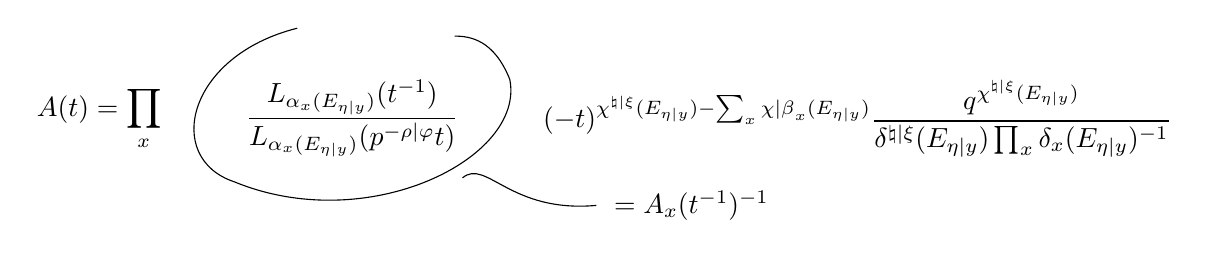
\begin{tikzpicture}[x=1cm,y=1cm]
\node[anchor=east] at (0,0) {$\displaystyle A(t)=\prod_x$};
\node at (2.3,0) {$\displaystyle\frac{L_{\alpha_x(E_{\unsure{\eta|y}})}(t^{-1})}{L_{\alpha_x(E_{\unsure{\eta|y}})}(p^{-\unsure{\rho|\varphi}}t)}$};
\node[anchor=west] at (4.6,0) {$\displaystyle(-t)^{\chi^{\unsure{\natural|\xi}}(E_{\unsure{\eta|y}})-\sum_x\unsure{\chi|\beta}_x(E_{\unsure{\eta|y}})}\frac{q^{\chi^{\unsure{\natural|\xi}}(E_{\unsure{\eta|y}})}}{\delta^{\unsure{\natural|\xi}}(E_{\unsure{\eta|y}})\prod_x\delta_x(E_{\unsure{\eta|y}})^{-1}}$};
\draw (1.6,1.15) .. controls (0.2,0.8) and (-0.1,-0.5) .. (0.8,-0.8) .. controls (2.5,-1.5) and (4.5,-0.5) .. (4.3,0.5) .. controls (4.1,1) and (3.8,1.05) .. (3.6,1.05);
\draw (3.7,-0.75) .. controls (4,-0.5) and (4.3,-1.2) .. (5.4,-1.1);
\node[anchor=west] at (5.5,-1.1) {$=A_x(t^{-1})^{-1}$};
\end{tikzpicture}}

\[
L_{\alpha_x(E_{\unsure{\eta|y}})}\left(\frac1{p^{\unsure{\rho|\varphi}}t}\right)=A_x(t)L_{\alpha_x(E_{\unsure{\eta|y}})}(t)
\]
\deleted{$\unsure{L_{\alpha_x(E)}}\quad L_{\alpha_x(E_{\unsure{\eta|y}})}($}

N.B. Ayant \unsure{coupé} $\lambda_x(\deleted{\unsure{\mu E}}\inserted{E_{\unsure{\eta|y}}})(t)$ \deleted{\unsure{en}} en \unsure{morceaux} ; on en perd le \uline{caractère additif}, Il vaut sans doute mieux ne pas \unsure{forcer} l'expression

\uline{Pb} a) Dans les cas géométriques classiques, construire les $\alpha_x(E_{\unsure{\eta|y}})$ pour déterminer les $\mu_x$, donc les $\lambda_x(E_{\unsure{\eta|y}})(t)$.
\diagram{\begin{tikzcd}[column sep=small,row sep=large]
\text{Déterminer en particulier} & \unsure{\chi|\beta}_x(E_{\unsure{\eta|y}}),\arrow[d,bend right] & \delta_x(E_{\unsure{\eta|y}}),\arrow[d,bend left]\\
\text{\parbox{7cm}{les \unsure{valeurs absolues} des \unsure{val.} propres de \unsure{Frobenius}.}} & \begin{gathered}\text{\unsure{invariant}}\\\text{\uuline{géom.}}\end{gathered} & \begin{gathered}\text{\unsure{invariant}}\\\text{\uuline{arithm.}}\end{gathered}\\
\text{\parbox{7cm}{b) Donner une formule genre \unsure{Chafarevitch} - Ogg pour}} & \chi^{\unsure{\natural|\xi}}(E_{\unsure{\eta|y}})\arrow[u,bend right] & \\
\text{c) Donner une formule pour} & & \delta^{\unsure{\natural|\xi}}(E_{\unsure{\eta|y}})\arrow[uu,bend right]
\end{tikzcd}}

\margin{54}
\scanpage{56}
\begin{center}4 - 36 -\hfill n\textsuperscript{o} 392\end{center}

Revenant à la démonstration de la prop. 19, on a, en vertu du lemme 4,
\[
\bigcap_{\underline{P}\in P(B)}R_{\underline{P}}=\bigcap_{\underline{p}\in P(A)}(R_{[A]})_{\underline{p}},
\]
et la conclusion résulte du n\textsuperscript{o} 2, th. 2.

PROPOSITION 20.- (i) \uline{Pour qu'un} $A$-\uline{module de type fini} $M$ \uline{soit pseudo-nul}, \uline{il faut et il suffit que} $M\otimes_A B$ \uline{soit un} $B$-\uline{module pseudo-nul}.

(ii) \uline{Si} $M$ \uline{est un} $A$-\uline{module de torsion de type fini}, $M\otimes_A B$ \uline{est un} $B$-\uline{module de torsion de type fini}, \uline{et l'on a} :
\[
(22)\qquad\unsure{\chi|\gamma}_B(M\otimes_A B)=i(\unsure{\chi|\gamma}_A(M)).
\]

(iii) \uline{Si} $M$ \uline{est un} $A$-\uline{module de type fini}, $M\otimes_A B$ \uline{est un} $B$-\uline{module de type fini}, \uline{et l'on a} :
\[
\begin{aligned}
(23)\qquad &c_B(M\otimes_A B)=i(c_A(M))\\
(24)\qquad &r_B(M\otimes_A B)=r_A(M).
\end{aligned}
\]

(i) Soient $\underline{P}$ un idéal premier de $B$, $\underline{p}=\underline{P}\cap A$ ; on a $(M\otimes_A B)_{\underline{P}}=M\otimes_A B_{\underline{P}}$, (chap. II, § 2, n\textsuperscript{o} 7, prop. 18), et d'autre part $M\otimes_A B_{\underline{P}}=(M\otimes_A A_{\underline{p}})\otimes_{A_{\underline{p}}}B_{\underline{P}}= {}=M_{\underline{p}}\otimes_{A_{\underline{p}}}B_{\underline{P}}$ ; la relation $M_{\underline{p}}=0$ est donc équivalente à $(M\otimes_A B)_{\underline{P}}=0$, (chap. II, § 4, n\textsuperscript{o} 4, lemme 4). Il suffit d'appliquer cette remarque à l'idéal $\underline{P}=(0)$ et aux idéaux $\underline{P}\in P(B)$ pour prouver (i), compte tenu du n\textsuperscript{o} 4, prop. 9.

Pour prouver (ii), nous utiliserons le lemme suivant :

LEMME 5.- \uline{Soient} $M_1$, $M_2$ \uline{deux} $A$-\uline{modules de type fini}, $f:M_1\longrightarrow M_2$ \uline{un homomorphisme injectif}. \uline{Alors le noyau de} $f\otimes1_B:M_1\otimes_A B\longrightarrow M_2\otimes_A B$ \uline{est pseudo-nul}.

Soit $\underline{p}$ un idéal premier de $A$ de hauteur $\le1$. On a $(M_i\otimes_A B)_{\underline{p}}=(M_i)_{\underline{p}}\otimes_{A_{\underline{p}}}B_{\underline{p}}$ $(i=1,2)$, (chap. II, § 2, n\textsuperscript{o} 7, prop. 18), et $(f\otimes1_B)_{\underline{p}}=f_{\underline{p}}\otimes1_{B_{\underline{p}}}$ ; l'hypothèse que $f$ est injectif entraîne qu'il en est de même de $f_{\underline{p}}$, (chap. II, § 1, n\textsuperscript{o} 4, th. 1) ; d'autre part, vu le choix de $\underline{p}$, $A_{\underline{p}}$ est un anneau principal et $B_{\underline{p}}$ un $A_{\underline{p}}$-module sans torsion de type fini, donc \uline{libre} ; on en conclut que $f_{\underline{p}}\otimes1_{B_{\underline{p}}}$ est

\margin{55}
\scanpage{57}
Sur la formule virtuelle \unsure{donnant} $D(E_{\unsure{\eta|y}}^{\unsure{\natural|\xi}})$, on lit
\[
\delta^{\unsure{\natural|\xi}}(E_{\unsure{\eta|y}})^{-1}=\delta^{\unsure{\natural|\xi}}(E_{\unsure{\eta|y}})p^{-\chi^{\unsure{\natural|\xi}}(E)(\unsure{\rho|\varphi}+1)}\prod_x\delta_x(\mu_x(E))
\]
Or
\[
\begin{aligned}
\delta(\mu_x(E))&=\delta(\alpha_x(E_{\unsure{\eta|y}}))^{-1}\bigl[\delta(\alpha_x(E_{\unsure{\eta|y}}))p^{-\unsure{\chi|\beta}_x(E_{\unsure{\eta|y}})(\unsure{\rho|\varphi}+1)}\bigr]^{-1}\\
&=\delta_x(E_{\unsure{\eta|y}})^{-2}q^{+\unsure{\chi|\beta}_x(E_{\unsure{\eta|y}})}
\end{aligned}
\]
d'où
\[
\unsure{\{}\prod_x\frac{\delta_x(E_{\unsure{\eta|y}})^2}{q^{\unsure{\chi|\beta}_x(E_{\unsure{\eta|y}})}}\unsure{\}}=\delta^{\unsure{\natural|\xi}}(E_{\unsure{\eta|y}})^2q^{\sum\unsure{\chi|\beta}_x(E_{\unsure{\eta|y}})}
\]
\[
\left\{\begin{aligned}
\frac{\delta^{\unsure{\natural|\xi}}(E_{\unsure{\eta|y}})^2}{q^{\chi^{\unsure{\natural|\xi}}(E)}}\deleted{\unsure{=q^{\chi^{\unsure{\natural|\xi}}(E)}}}&=\prod_x\frac{\delta_x(E_{\unsure{\eta|y}})^2}{q^{\unsure{\chi|\beta}_x(E_{\unsure{\eta|y}})}}\qquad\text{\unsure{ou encore}}\\
\Vert&\\
\varepsilon^{\unsure{\natural|\xi}}(E_{\unsure{\eta|y}})^2&=\prod_x\frac{\delta_x(E_{\unsure{\eta|y}})^2}{q^{\unsure{\chi|\beta}_x(E_{\unsure{\eta|y}})}}
\end{aligned}\right.
\]

\diagram{\begin{tikzcd}[column sep=large,row sep=large]
\varepsilon^{\unsure{\natural|\xi}}(E_{\unsure{\eta|y}})\arrow[d,equal] & {=\displaystyle\pm\prod_x\frac{\delta_x(E_{\unsure{\eta|y}})}{q^{\unsure{\chi|\beta}_x(E_{\unsure{\eta|y}})/2}}=\left(\prod_x\frac{\delta_x(E_{\unsure{\eta|y}})}{p^{\unsure{\rho|\varphi}\unsure{\chi|\beta}_x(E_{\unsure{\eta|y}})/2}}\right)\frac1{p^{\chi/2}}}\\
\displaystyle\frac{\delta^{\unsure{\natural|\xi}}(E_{\unsure{\eta|y}})}{q^{\chi^{\unsure{\natural|\xi}}(E_{\unsure{\eta|y}})/2}} & \boxed{\chi=\sum_x\unsure{\chi|\beta}_x(E_{\unsure{\eta|y}})}\arrow[u,bend right]\arrow[dl,bend left]\\
{\varepsilon^{\unsure{\natural|\xi}}(E_{\unsure{\eta|y}})=\displaystyle\pm\left(\prod_x\varepsilon_x(E_{\unsure{\eta|y}})\right)p^{-\chi/2}} &
\end{tikzcd}}

\margin{56}
\scanpage{58}
\begin{center}4 - 35 -\hfill n\textsuperscript{o} 392\end{center}

libre de $R$ tel que $R/M$ soit un $B$-module de torsion ; comme $M_{[A]}$ est somme directe de $r_B(R)$ $A$-modules isomorphes à $B$, on a, (prop. 16, (i)), $c_A(M_{[A]})= {}=r_B(R).c_A(B)$. D'autre part, $c_A((R/M)_{[A]})=-c_A(N(\unsure{\chi|\gamma}_B(R/M)))$ en vertu de (19) ; mais par définition de l'homomorphisme $N:C(B)\longrightarrow C(A)$, on a $c_A(N(d))=N(c_B(d))$ pour tout $d\in D(B)$, et comme $c_B(\unsure{\chi|\gamma}_B(R/M))=-c_B(R)$ par définition, on a finalement $c_A((R/M)_{[A]})=N(c_B(R))$ ; il suffit alors d'appliquer la prop. 16, (i) pour obtenir (20).

PROPOSITION 19.- \uline{Soit} $R$ \uline{un} $B$-\uline{module de type fini}. \uline{Pour que} $R$ \uline{soit réflexif}, \uline{il faut et il suffit que} $R_{[A]}$ \uline{soit un} $A$-\uline{module réflexif}.

Il est clair que pour que $R$ soit un $B$-module sans torsion, il faut et il suffit que $R_{[A]}$ soit un $A$-module sans torsion. On peut donc supposer que $R$ est un réseau de $W=R\otimes_B L$ par rapport à $B$. Nous utiliserons le lemme suivant :

LEMME 4.- \uline{Soit} $W$ \uline{un espace vectoriel de dimension finie sur} $L$ \uline{et soit} $R$ \uline{un réseau de} $W$ \uline{par rapport à} $B$. \uline{Pour tout} $\underline{p}\in P(A)$, \uline{on a alors} $(R_{[A]})_{\underline{p}}=\bigcap_{\underline{P}\mid\underline{p}}R_{\underline{P}}$.

En effet, si $S=A-\underline{p}$, les idéaux premiers de l'anneau $S^{-1}B$ sont engendrés par les idéaux premiers de $B$ ne rencontrant pas $S$, autrement dit les idéaux $\underline{P}_i$, $(1\le i\le m)$, au-dessus de $\underline{p}$ et l'idéal $(0)$ ; cela montre que $S^{-1}B$ est un anneau semi-local dont les idéaux maximaux sont les $\underline{m}_i=\underline{P}_i(S^{-1}B)$ pour $1\le i\le m$ ; en outre l'anneau local $(S^{-1}B)_{\underline{m}_i}$ est isomorphe à $B_{\underline{P}_i}$, (chap. II, § 2, n\textsuperscript{o} 5, prop. 11), donc est un anneau de valuation discrète. L'anneau $S^{-1}B$ est par suite un anneau de Dedekind, (§ 3, n\textsuperscript{o} 2, th. 1, e)), et comme il est semi-local, il est principal, (§ 3, n\textsuperscript{o} 2, prop. 1). Cela étant, $(R_{[A]})_{\underline{p}}$ est égal à $S^{-1}R$, considéré comme $A_{\underline{p}}$-module ; d'après ce qui précède, $S^{-1}R$ est un réseau \uline{libre} de $W$ par rapport à $S^{-1}B$ et on peut par suite lui appliquer le th. 2 du n\textsuperscript{o} 2, qui donne $S^{-1}R=\bigcap_i(S^{-1}R)_{\underline{m}_i}$ ; mais $(S^{-1}R)_{\underline{m}_i}=R_{\underline{P}_i}$, ce qui prouve le lemme.

\margin{57}
\scanpage{59}
On voit donc que c) est \unsure{ramené} (\uline{modulo un signe}) au cas de b), donc à déterminer $\chi^{\unsure{\natural|\xi}}(E_{\unsure{\eta|y}})$. Or cette détermination est faite, en utilisant les représentations d'Artin \unsure{-{}-{}-{}-|....}

\margin{58}
\scanpage{60}
\begin{center}4 - 34 -\hfill n\textsuperscript{o} 392\end{center}

entier sur $A$, il n'y a pas d'autre idéal que $0$ au-dessus de l'idéal $0$ de $A$, (chap. V, § 2, n\textsuperscript{o} 1, cor. 1 de la prop. 1), donc il revient au même de dire que $\underline{a}\ne0$ ou que $\underline{b}\ne0$.

(i) En vertu de ce qui précède, on peut se borner au cas où $R$ est un $B$-module de torsion. Si $\underline{b}$ est contenu dans un idéal premier $\underline{P}\in P(B)$, $\underline{a}$ est contenu dans $\underline{P}\cap A=\underline{p}$, qui est de hauteur $1$. Inversement, si $\underline{a}$ est contenu dans un idéal premier $\underline{p}\in P(A)$, il existe un idéal premier $\underline{P}$ de $B$ qui contient $\underline{b}$ et est au-dessus de $\underline{p}$, (chap. V, § 2, n\textsuperscript{o} 1, cor. 2 du th. 1). L'assertion (i) résulte de ces remarques et du n\textsuperscript{o} 4, prop. 9.

(ii) Pour tout $B$-module de torsion de type fini $R$, posons $\varphi(R)=\unsure{\chi|\gamma}_A(R_{[A]})$ ; il est clair que, (pour les $B$-modules de torsion de type fini), $\varphi$ vérifie les conditions 1) et 2) de la prop. 11 du n\textsuperscript{o} 5, (compte tenu de (i)). Il existe par suite un homomorphisme $\unsure{\vartheta|\theta}:D(B)\longrightarrow D(A)$ tel que $\varphi(R)=\unsure{\vartheta|\theta}(\unsure{\chi|\gamma}_B(R))$ pour tout $B$-module de torsion $R$ de type fini. L'homomorphisme $\unsure{\vartheta|\theta}$ est déterminé par sa valeur pour tout $B$-module de la forme $B/\underline{P}$ où $\underline{P}\in P(B)$, puisque $\unsure{\chi|\gamma}_B(B/\underline{P})=\underline{P}$. Or, pour tout idéal premier $\underline{q}\ne\underline{p}=\underline{P}\cap A$ dans $P(A)$, on a $\underline{q}\not\subset\underline{P}$, donc $(B/\underline{P})_{\underline{q}}=0$. D'autre part, si on pose $S=A-\underline{p}$, $\underline{P}.S^{-1}B$ est un idéal maximal de $S^{-1}B$ et $(B/\underline{P})_{\underline{p}}=S^{-1}B/\underline{P}.S^{-1}B$ est isomorphe au corps des fractions de $B/\underline{P}$, c'est-à-dire au corps résiduel de $v_{\underline{P}}$ ; sa longueur en tant que $A_{\underline{p}}$-module est donc $f_{\underline{P}/\underline{p}}$ ; ce qui prouve que $\unsure{\vartheta|\theta}=N$, (n\textsuperscript{o} 5, déf. 4).

(iii) Si $T$ est le sous-module de torsion de $R$, $T_{[A]}$ est le sous-module de torsion de $R_{[A]}$, et $(R/T)_{[A]}=R_{[A]}/T_{[A]}$ ; pour prouver (21), on peut donc se borner au cas où $R$ est sans torsion. Alors $R$ est identifié à un sous-$B$-module de $R_{(L)}$, et contient une base $(e_i)_{1\le i\le m}$ de $R_{(L)}$ sur $L$. Si $(b_j)_{1\le j\le n}$ est une base de $L$ sur $K$ formée d'éléments de $B$, les $b_je_i$ constituent une base de $R_{(L)}$ sur $K$, formée d'éléments de $R$, d'où (21). Soit d'autre part $M$ un sous-$B$-module

\margin{59}
\scanpage{61}
Cohomologie à l'infini

$\unsure{\mathbb{R}|\mathbf{R}}^*_{\infty}f(F)$ pour $f$ compactifié en $\bar f$

On regarde la suite exacte
\diagram{\begin{tikzcd}[column sep=large]
\unsure{\mathbb{R}|\mathbf{R}}i_!(F) \arrow[r] & \unsure{\mathbb{R}|\mathbf{R}}\unsure{f|i}_*(F) \arrow[r] & \unsure{\mathbb{R}|\mathbf{R}}i_*(F)|Y \arrow[ll,bend right=30]
\end{tikzcd}}
d'où en appliquant $\unsure{\mathbb{R}|\mathbf{R}}\bar f_*$ une suite exacte
\fbox{\diagram{\begin{tikzcd}[column sep=small]
\ldots \arrow[r] & \unsure{\mathbb{R}|\mathbf{R}}^i f_!(F) \arrow[r] & \unsure{\mathbb{R}|\mathbf{R}}^i f_*(F) \arrow[r] & \unsure{\mathbb{R}|\mathbf{R}}^i_{\infty}f(F) \arrow[r] & \unsure{\mathbb{R}|\mathbf{R}}^{\unsure{i-1|i+1}}f_!(F) \arrow[r] & \ldots
\end{tikzcd}}}
en posant
\[
\unsure{\mathbb{R}|\mathbf{R}}^i_{\infty}f(F)=\unsure{\mathbb{R}|\mathbf{R}}^i\bar f_*(\unsure{\mathbb{R}|\mathbf{R}}i_*(F)|Y)
\]

On peut aussi considérer la suite exacte \inserted{\unsure{en cat. dérivée}} pour $\deleted{\unsure{\mathbb{R}|\mathbf{R}}i_*(F)}\inserted{\unsure{\mathbb{R}|\mathbf{R}}i_!(F)}$ sur $\bar X$, et l'ouvert $\unsure{X}$ et $Y=\bar X-X$, \deleted{\unsure{qui associe}}
\diagram{\begin{tikzcd}[column sep=large]
\unsure{\mathbb{R}|\mathbf{R}}j^!(\unsure{\mathbb{R}|\mathbf{R}}i_!(F)) \arrow[r] & \unsure{\mathbb{R}|\mathbf{R}}i_!(F) \arrow[r,no head] & \unsure{\mathbb{R}|\mathbf{R}}i_*(F) \arrow[ll,bend right=30]
\end{tikzcd}}
\deleted{\diagram{\begin{tikzcd}[column sep=large]
\unsure{\mathbb{R}|\mathbf{R}}^i_{\unsure{\infty}} \arrow[r,no head] & \unsure{\mathbb{R}|\mathbf{R}}^i f_!(F) \arrow[r] & \unsure{\mathbb{R}|\mathbf{R}}^i f_*(F) \arrow[r] & {}
\end{tikzcd}}}
et \unsure{au décalage d'une unité près}, $\unsure{\mathbb{R}|\mathbf{R}}i_*(F)|Y$ est \unsure{fourni} par $\unsure{\mathbb{R}|\mathbf{R}}j^!\unsure{\mathbb{R}|\mathbf{R}}i_!(F)$ .---

\margin{60}
\scanpage{62}
\begin{center}6 - 45 -\hfill n\textsuperscript{o} 392\end{center}

d) Déduire de c) un exemple d'anneau de valuation discrète $A$ et d'une extension séparable $L$ de $K$ tel que $B$ ne soit de la forme $A[x]$ pour aucun $x\in B$, (partir d'une extension cyclotomique de $Q$, en utilisant l'exerc. 11 du chap. VI, § 8).

8)\quad a) Soient $A$ un anneau de Dedekind, $K$ son corps des fractions, $L$ une extension finie séparable de $K$, $B$ la fermeture intégrale de $A$ dans $L$. On suppose que pour tout idéal premier $\underline P$ de $B$, le corps résiduel de $B$ en $\underline P$ soit séparable sur celui de $A$ en $\underline P\cap A$. Montrer qu'il existe un élément $x\in B$ tel que le $B$-module $\Omega_A(B)$ des différentielles de $B$ sur $A$ soit engendré par $\mathrm{d}x$.

b) Donner un exemple d'un anneau de valuation discrète complet $A$, et d'une extension séparable $L$ du corps des fractions $K$ de $L$, tels que si $B$ est la fermeture intégrale de $A$ dans $L$, $\bar K$ et $\bar L$ les corps résiduels de $A$ et $B$ respectivement, $\bar L$ soit une extension radicielle non monogène de $\bar K$, (procéder comme dans le chap. VI, § 8, exerc. 10). Pour une telle extension, montrer que le $B$-module $\Omega_A(B)$ n'est pas monogène.

\begin{center}-:-:-:-\end{center}
\margin{61}
\scanpage{63}
$L(t)$ une fonction rat. en $t$, \deleted{\unsure{poids}} $q=p^{\unsure{f}}$
\[
L\left(\frac1{qt}\right)=A(t)L(t)\qquad A(t)\text{ de ``niveau'' inférieur}
\]
On veut simplifier l'équation fonctionnelle, en posant
\[
L'(t)=\lambda(t)L(t)
\]
d'où
\[
\begin{aligned}
L'\left(\frac1{qt}\right)&=\lambda\left(\frac1{qt}\right)L\left(\frac1{qt}\right)=\lambda\left(\frac1{qt}\right)A(t)L(t)\\
&=\lambda\left(\frac1{qt}\right)\lambda(t)^{-1}A(t)L'(t)
\end{aligned}
\]
et on aimerait obtenir $L'(\frac1{qt})=cL'(t)$, i.e.
\[
\frac{\lambda(\frac1{qt})}{\lambda(t)}=cA(t)^{-1}
\]
Si on trouve un tel $\lambda$, tout autre $\lambda'(t)=\alpha(t)\lambda(t)$ \inserted{avec une $\unsure{c^{te}}$ $c'$} est déterminé par $\alpha$ satisfaisant
\[
\frac{\alpha(\frac1{qt})}{\alpha(t)}=\frac{c'}c\qquad\text{i.e.}\quad\alpha\left(\frac1{qt}\right)=a\alpha(t)
\]
\uline{avec $a$ une $\unsure{c^{te}}$,}
\figure{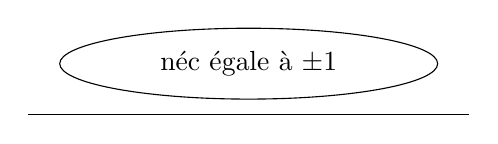
\begin{tikzpicture}
\node (a) at (0,0) {\unsure{néc} \unsure{égale} à $\pm1$};
\draw (0,0) ellipse (2.4 and .45);
\draw (-2.8,-.65)--(2.8,-.65);
\end{tikzpicture}}
\margin{\uline{donc dans l'équation fonctionnelle \unsure{multiplic.} $c$ est un signe}}

Faisons opérer le groupe $\deleted{\unsure{G}}$ $\unsure{\mathbf{Z}|Z}/2\unsure{\mathbf{Z}|Z}$ sur les \inserted{\unsure{gr. mult.}} fonctions rationnelles \inserted{$\ne0$}, par la substitution $t\longmapsto\frac1{qt}$. Alors (pour $c$ donné) la question \unsure{de trouver} $\lambda$

\margin{62}
\scanpage{64}
\begin{center}6 - 35 -\hfill n\textsuperscript{o} 392\end{center}

9) Soient $k$ un corps, $A$ l'anneau de polynômes $k[X,Y]$. Dans le $A$-module $M=A^2$, on considère la forme linéaire $f$ telle que $f(e_1)=X$, $f(e_2)=Y$, ($(e_1,e_2)$ étant la base canonique). Montrer que le noyau $L$ de $f$ est un $A$-module libre monogène, mais que le quotient $M/L$, (qui est isomorphe à un idéal de $A$), n'est pas réflexif.

10) Soit $A$ un anneau commutatif. Pour tout sous-module $R$ d'un $A$-module libre de type fini $L=A^n$, on désigne par $\underline c_1(R)$ l'idéal engendré par les $\langle x,x^*\rangle$, où $x$ parcourt $R$ et $x^*$ parcourt le dual $L^*$ ; on pose $\underline c_k(R)=\underline c_1(\operatorname{Im}(\bigwedge^k R))$, $\operatorname{Im}(\bigwedge^k R)$ étant l'image canonique de la puissance extérieure $k$-ème de $R$ dans $\bigwedge^k L$. Si $R_1\subset R_2$ sont deux sous-modules de $L$, on a $\underline c_k(R_1)\subset\underline c_k(R_2)$ pour tout $k$.

a) Soit $M$ un $A$-module de type fini : $M$ est isomorphe à un module quotient $L/R$, où $L=A^n$ pour un $n$ convenable. Montrer que la suite d'idéaux $(\underline a_k)_{k\geq0}$ telle que $\underline a_k^{\unsure{\prime}}=\underline c_{n-k}(R)$ pour $k\leq n$ et $\underline a_k=A$ pour $k>n$, est indépendante de l'expression de $M$ sous la forme $L/R$. (Considérer d'abord le cas où $L/R$ et $L'/R'$ sont isomorphes ; remarquer ensuite que $A^n/R$ est isomorphe à $A^{n+h}/(R\times A^h)$ pour tout $h>0$). On pose $\underline d_k(M)=\underline a_k$ pour tout $k\geq0$, et on dit que ce sont les \uline{idéaux déterminantiels} associés à $M$. On a $\underline d_k(M)\subset\underline d_{k+1}(M)$ pour $k\geq0$.

b) Si $A$ est un anneau principal et $M=L/R$ où $L$ est libre de type fini, montrer que les idéaux $\underline c_{k+1}(R)(\underline c_k(R))^{-1}$ sont les \uline{facteurs invariants} de $R$ dans $L$.

c) Soit $r=\unsure{\gamma|g}(M)$ le plus petit des cardinaux des systèmes de générateurs de $M$, et soit $r_0$ le plus petit entier $h$ tel que $\underline d_h(M)=A$. Montrer que $r_0\leq r$ et donner un exemple où $r_0<r$, (prendre pour $A$ un anneau de Dedekind).

d) Si $\underline a$ est l'annulateur de $M$, montrer que l'on a $\underline d_0(M)\subset\underline a$ et $\underline a^{r-k}\subset\underline d_k(M)$ pour $k\leq r=\unsure{\gamma|g}(M)$.

e) On suppose que $M$ est somme directe de sous-modules $M_i$, $(1\leq i\leq h)$. Montrer que l'on a :
\[
\underline d_k(M)=\sum\underline d_{k_1}(M_1)\ldots\underline d_{k_h}(M_h)
\]
où la somme est étendue aux suites finies $(k_i)_{1\leq i\leq h}$ telles que $\sum_{i=1}^h k_i=k$.

f) Si $N$ est un sous-module de type fini de $M$, on a $\underline d_k(M/N)\subset\underline d_k(M)$ pour tout $k\geq0$. Montrer que l'on a :
\[
\sum_{j=0}^k\underline d_j(N)\underline d_{k-j}(M/N)\subset\underline d_k(M).
\]
\margin{63}
\scanpage{65}
\deleted{\unsure{équivaut à celle qu'on va écrire}}
\[
\deleted{\boxed{\underline\lambda^{\unsure{g|\sigma}}\lambda^{-1}=}}
\]

Il y a une solution triviale
\[
\lambda=\frac1L\qquad\text{i.e.}\quad L'(t)=1.
\]
Mais nous désirons imposer que $\lambda\deleted{\unsure{L}}$ soit de ``niveau'' \unsure{strict.} inf. à $L$.

Pour préciser ce point, nous supposerons
\deleted{\fbox{$L(0)=1$,} que les racines et pôles de $L$ sont en valeurs absolues de la forme
\[
p^{-\frac i2}\quad\text{avec}\quad \unsure{4|2}\rho\leq i\leq\unsure{4|2}\rho+2n\qquad\text{i.e.}\quad\rho\leq\frac i2\leq\rho+n,
\]
\deleted{et \unsure{modulo multiplication} par des puissances de $p^{1/2}$, des valeurs \uuline{propres inverses}}
(et on veut se restreindre aux $\lambda$ ayant \uline{la \unsure{$=$|même} propriété}, \deleted{et de plus} (de poids compris entre $\rho$ et $\rho+n$) et de plus de ``niveau'' \deleted{$\unsure{\rho+n+1}$}}

\margin{\unsure{et sont de la forme} $(p^{1/2})^{\unsure{\nu|n}}\xi_i$, où $\nu$ un entier, $\xi_i$ un \uline{entier alg.}}

\diagram{\begin{tikzcd}[column sep=small]
L(t)={} & {L_\rho(t)\ldots L_{\rho\deleted{\unsure{\delta|2}}+n}(t)} \arrow[loop below,distance=1.4em,"{\deleted{\unsure{=L}}}"'] & {L'_{\rho+n-1}(pt)L'_{\rho+n-2}(p^2t)\ldots L'_\rho(p^nt)}
\end{tikzcd}}
\deleted{\unsure{et de}}
où les valeurs propres inverses des $\unsure{L_{i/2}|L_i}$ sont des entiers alg en \unsure{val.} absolue $p^{i/2}$, et de \unsure{$=$|même} pour $L'_i$ (donc $L'_{\rho+n-i}(p^it)$ a des valeurs propres inverses qui sont des entiers alg de val. absolue $p^{\frac{\rho+n-i}{2}}p^i=p^{\frac{\rho+n+i}{2}}$.

\margin{64}
\scanpage{66}
\begin{center}6 - 34 -\hfill n\textsuperscript{o} 392\end{center}

6) Soient $k$ un corps, $B$ l'anneau de polynômes $k[X,Y]$, $A$ le sous-anneau $k[X^2,XY,Y^2]$ de $B$.

a) Montrer que $A$ est un anneau noethérien intégralement clos et que $B$ est un $A$-module de type fini.

b) Montrer que l'idéal $\underline p=AX^2+AXY$ de $A$ est un idéal premier de hauteur 1, (donc divisoriel), mais que le $B$-module $\underline p\otimes_A B$ a un module de torsion $\ne0$ et n'est donc pas réflexif ; l'idéal $\underline pB$ de $B$ n'est pas divisoriel, l'application canonique $\underline p\otimes_A B\longrightarrow\underline pB$ n'est pas injective et $\underline p$ n'est pas un $A$-module plat.

7) Soient $A$ un anneau noethérien intégralement clos, $E$ un $A$-module sans torsion de type fini, $E^*$ son dual.

a) Montrer que l'homomorphisme canonique $E^*\otimes_A E\longrightarrow\operatorname{End}_A(E)$ est un pseudo-isomorphisme.

b) Déduire de a) que pour que $E$ soit un $A$-module projectif, il faut et il suffit que $E^*\otimes_A E$ soit un $A$-module réflexif. (Remarquer que si $E^*\otimes_A E$ est réflexif, l'homomorphisme canonique $E^*\otimes_A E\longrightarrow\operatorname{End}_A(E)$ est bijectif).

*8) Soient $A$ un anneau noethérien intégralement clos, $M_1$, $M_2$ deux $A$-modules de type fini.

a) Montrer que les $A$-modules $\operatorname{Tor}_i^A(M_1,M_2)$, $\operatorname{Ext}_A^i(M_1,M_2)$ sont pseudo-nuls pour $i\geq2$, (se ramener au cas où $A$ est principal).

b) Si $M_1$ est sans torsion, montrer que $\operatorname{Tor}_1^A(M_1,M_2)$ et $\operatorname{Ext}_A^1(M_1,M_2)$ sont pseudo-nuls, (même méthode).

c) Si $M_1$ est un $A$-module de torsion, montrer que l'on a, (avec les notations du n\textsuperscript{o}\quad) :
\[
\begin{aligned}
\unsure{\chi|\gamma}(M_1\otimes_A M_2)-\unsure{\chi|\gamma}(\operatorname{Tor}_1^A(M_1,M_2))&=r(M_2)\unsure{\chi|\gamma}(M_1)\\
\unsure{\chi|\gamma}(\operatorname{Hom}_A(M_1,M_2))-\unsure{\chi|\gamma}(\operatorname{Ext}_A^1(M_1,M_2))&=-r(M_2)\unsure{\chi|\gamma}(M_1)\\
\unsure{\chi|\gamma}(\operatorname{Hom}_A(M_2,M_1))-\unsure{\chi|\gamma}(\operatorname{Ext}_A^1(M_2,M_1))&=r(M_2)\unsure{\chi|\gamma}(M_1)
\end{aligned}
\]

d) Montrer que pour tout couple de $A$-modules de type fini $M_1$, $M_2$, on a :
\[
\begin{aligned}
c(M_1\otimes_A M_2)-c(\operatorname{Tor}_1^A(M_1,M_2))&=r(M_1)c(M_2)+r(M_2)c(M_1)\\
c(\operatorname{Hom}_A(M_1,M_2))-c(\operatorname{Ext}_A^1(M_1,M_2))&=r(M_1)c(M_2)-r(M_2)c(M_1).\quad *
\end{aligned}
\]
\margin{65}
\scanpage{67}
Ceci posé, on \deleted{\unsure{veut}} se permet de ``corriger'' par des $\lambda$ \unsure{seulement} de la forme
\[
\begin{gathered}
\lambda_\rho(t)\ldots\lambda_{\rho+n-1}(t)\lambda_{\rho+n-2}(pt)\lambda_{\rho+n-1}(pt)\lambda_{\rho+n-2}(p^2t)\\
\ldots\lambda_\rho(p^nt)
\end{gathered}
\]
donc de poids entre $\rho$ et $\unsure{\rho+2n|\rho+n}$ comme $L$, mais de \uline{niveau} $\leq\rho+n-1$ (et non seulement $\leq\rho+n$ comme $L$)

\deleted{Si le terme $L_{\rho+n}$}

Mais supposons de plus que $A(t)$ lui-\unsure{$=$|même} est de \deleted{\unsure{même}} ce type.

\diagram{\begin{tikzcd}[row sep=large]
{\begin{gathered}
L\left(\frac1{p^{\unsure{n-\rho|n+\rho}}t}\right)=L'_\rho\left(\frac1{p^\rho t}\right)L'_{\rho+1}\left(\frac1{p^{\rho+1}t}\right)\ldots L'_{\rho+n-1}\left(\frac1{p^{\unsure{n-\rho-1|n+\rho-1}}t}\right)\\
L_{\rho+n}\left(\frac1{p^{\rho+n}t}\right)L_{\rho+n-1}\left(\frac1{p^{\unsure{n-\rho|n+\rho}}t}\right)\ldots L_\rho\left(\frac1{p^{\unsure{n-\rho|n+\rho}}t}\right)
\end{gathered}} \arrow[dd,no head,out=190,in=180,looseness=1.8]\\
{\begin{gathered}\text{De plus, on suppose que chaque }L_i\text{ et }L'_i\text{ a}\\\text{une équation fonctionnelle du type correspondant}\end{gathered}}\\
{\begin{aligned}
={}&\delta'_\rho t^{\chi'_\rho}L'_\rho(t)\ldots\delta'_{\rho+n-1}t^{\chi'_{\rho+n-1}}L'_{\rho+n-\unsure{i|1}}(t)\\
&\unsure{\llcorner}\delta_{\rho+n}t^{\chi_\rho}L_{\rho+n}(t)\delta_{\rho+n-1}t^{\chi_{\rho+n-1}}L_{\rho+n-1}(pt)\\
&\ldots\delta_\rho t^{\chi_\rho}L_\rho(p^nt)\\
={}&\delta t^\chi L'_\rho(t)\ldots L'_{\rho+n-1}(t)L_{\rho+n}(t)L_{\rho+n-1}(\unsure{qt|pt})\ldots L_\rho(\unsure{q^nt|p^nt})
\end{aligned}}
\end{tikzcd}}

\margin{66}
\scanpage{68}
\begin{center}6 - 33 -\hfill n\textsuperscript{o} 392\end{center}
\begin{center}§ 4.\end{center}

1) Soient $A$ un anneau noethérien intégralement clos, $V$ un espace vectoriel de dimension finie sur le corps des fractions de $A$. Montrer que si $(M_\lambda)$ est une famille quelconque de réseaux réflexifs de $V$ contenant toutes un même réseau $N$, le réseau $M=\bigcap_\lambda M_\lambda$ est réflexif, (considérer les réseaux associés $M_\lambda^*$).

*2) Soient $A$ un anneau noethérien intégralement clos, $E$, $F$ deux $A$-modules de type fini. On suppose que $E$ est sans torsion, que $\operatorname{Hom}_A(E,F)$ est réflexif et que $\operatorname{Ext}_A^1(E,F)=0$. Montrer alors que $F$ est réflexif. (Prouver d'abord que $F$ est sans torsion ; si $T=F^{**}/c_F(F)$, calculer de deux manières $\operatorname{Ass}(\operatorname{Hom}_A(E,T))$ en utilisant la suite exacte :
\diagram{\begin{tikzcd}
0 \arrow[r] & \operatorname{Hom}(E,F) \arrow[r] & \operatorname{Hom}(E,F^{**}) \arrow[r] & \operatorname{Hom}(E,T) \arrow[r] & 0
\end{tikzcd}}
et le chap. IV, § 1, n\textsuperscript{o}\quad, prop.\quad). *

3) Soient $A$ un anneau noethérien intégralement clos, $K$ son corps des fractions, $M$ un réseau réflexif d'un espace vectoriel $V$ de dimension finie sur $K$, $L$ un réseau \uline{libre} de $V$ contenant $M$. Montrer qu'il existe un réseau libre $L_1$ de $V$ tel que $M=L\cap L_1$. (Considérer l'ensemble fini $I$ des idéaux premiers $\underline p$ de hauteur 1 de $A$ tels que $L_{\underline p}\ne M_{\underline p}$, et l'anneau principal $S^{-1}A$, où $S=\bigcap_{\underline p\in I}(A-\underline p)$ ; montrer qu'il existe un réseau libre $L_0$ de $V$ tel que $M_{\underline p}=(L_0)_{\underline p}$ pour tout $\underline p\in I$, et un $s\in S$ tel que $M\subset s^{-1}L_0=L_1$).

4) Soient $k$ un corps, $A$ l'anneau de polynômes $k[X,Y]$.

a) Soit $(e_1,e_2)$ la base canonique du $A$-module $A^2$, et soit $E$ le sous-$A$-module de $A^2$ engendré par $(X-Y)e_1$, $e_1+Xe_2$ et $e_1+Ye_2$ ; soit $F$ le sous-module monogène de $E$ engendré par $(X-Y)^2e_1$. Montrer que le $A$-module $M=E/F$ n'est pas somme directe de son sous-module de torsion et d'un module sans torsion.

b) Montrer que le $A$-module de torsion $A/AXY$ n'est pas somme directe de sous-modules monogènes de la forme $A/\underline P_i^{n_i}$, où les $\underline P_i$ sont des idéaux premiers de hauteur 1.

5) Soient $A$ un anneau noethérien intégralement clos, $M$ un $A$-module de type fini. Montrer que si $\underline a$, $\underline b$ sont deux idéaux de $A$, le $A$-module $((\underline aM)\cap(\underline bM))/(\underline a\cap\underline b)M$ est pseudo-nul ; donner un exemple où il n'est pas nul.

\margin{67}
\scanpage{69}
\deleted{\unsure{On peut}}
\[
\frac{L(\frac1{qt})}{L(t)}=\delta t^\chi
\left[\frac{L'_\rho(t)\,\unsure{--}}{L'_\rho(p^nt)}\ldots\frac{L'_{\rho+n-1}(t)}{L'_{\rho+n-1}(pt)}\right]
\left[\frac{L_{\rho+n-1}(pt)}{L_{\rho+\unsure{n-1|n}}(t)}\deleted{\unsure{L_\rho}}\ldots\frac{L_\rho(p^nt)}{L_\rho(t)}\right]
\]
\[
A(t)=\delta t^\chi\prod_i\frac{L'_i(t)}{L'_i(p^{\rho+n-i}t)}\prod_i\frac{L^{\unsure{\prime}}_{\unsure{i|\rho}}(\unsure{p|q}^{\rho+n-i}t)}{L^{\unsure{\prime}}_i(t)}
\]

\figure{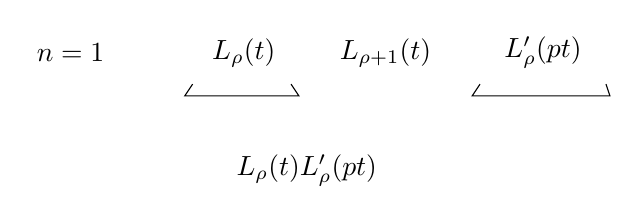
\begin{tikzpicture}
\node at (-4,0) {$n=1$};
\node at (-1.8,0) {$L_\rho(t)$};
\node at (0,0) {$L_{\rho+1}(t)$};
\node at (2,0) {$L'_\rho(pt)$};
\draw (-2.45,-.4)--(-2.55,-.55)--(-1.1,-.55)--(-1.2,-.4);
\draw (1.2,-.4)--(1.1,-.55)--(2.85,-.55)--(2.8,-.4);
\node at (-1,-1.5) {$L_\rho(t)L'_\rho(pt)$};
\end{tikzpicture}}

\margin{68}
\scanpage{70}
\begin{center}6 - 32 -\hfill n\textsuperscript{o} 392\end{center}

26) Soient $A$ un anneau factoriel, $K$ son corps des fractions. Pour que des éléments $f_i$, $(1\leq i\leq r)$, de $B=A[X_1,\ldots,X_n]$ soient tels que l'idéal $\sum_{i=1}^r Bf_i$ soit égal à $B$, il faut et il suffit qu'il existe des polynômes $v_i$, $(1\leq i\leq r)$, de $K[X_1,\ldots,X_n]$ tels que $\sum_{i=1}^r v_i f_i=1$ et qui vérifient en outre la condition suivante : si l'on pose $v_i=w_i/d$, où $d\in A$, les polynômes $w_i$ appartiennent à $A[X_1,\ldots,X_n]$ et le p. g. c. d. de l'ensemble des coefficients de tous les $w_i$, $(1\leq i\leq r)$, est égal à 1, alors, pour tout élément extrémal $p$ de $A$ divisant $d$, l'idéal engendré par les classes des $f_i$ dans l'anneau $(A/Ap)[X_1,\ldots,X_n]$ est cet anneau tout entier.

\begin{center}-:-:-:-\end{center}
\margin{69}
